\documentclass{article}

\usepackage[english]{babel}
\usepackage{microtype}
\usepackage{graphicx}
\usepackage{wrapfig}
\usepackage{enumitem}
\usepackage{fancyhdr}
\usepackage{amsmath}
\usepackage{chemformula}
\usepackage{index}
\usepackage{hyperref}
\usepackage[margin=1.0in]{geometry}
\usepackage{qtree}
\usepackage{float}

\begin{document}
\title{Summary: The Immune System}
\author{Dowland Aiello}
\date{}

\maketitle
\tableofcontents
\fancyhf{}

\newpage

\section{Categorization of immunities}

The \textbf{immune system} prevents hummans from constantly falling ill as a result
of exposure to \textbf{pathogens}---bacteria, fungi, viruses, etc\ldots--- in our
environment. More specifically, an \emph{inherent} or \textbf{innate immunity}
exists in all animals that are active even before infection takes place.

In the case of the invertebrate, innate immunity is the only mode of infection
deterrent available to the host. Yet, the innate immunities that invertebrates
posess are often effective in comabing infection. For example, externally, an
invertebrate has an exoskeleton, which keeps out bacteria and viruses through a
simple physical barrier. Internally, antimicrobial molecules in conjunction
with chemically unhospitable conditions lower the chance of infection.
Furthermore, generalized immune cells exist within the organism that are
capable of digesting foreign substances (i.e., pathogens that have already
entered the body).

In contrast to invertebrates, vertebrates have both \emph{innate} and
\textbf{adaptive immune} systems. Some innate immune systems posessed
by humans include:

\begin{itemize}
	\item Skin and mucous membranes
	\item Microbiota on the skin and mucous membranes
	\item Cilia placed throughout airways
	\item \textbf{Natural killer cells}: cells that recognize canerous or
		infected cells and release chemicals that result in their death
	\item \textbf{Phagocytes}
	\item \textbf{Defensive proteins} (e.g., interferons which interfere with
		viral infections)
	\item \textbf{Complement system}: a group of different proteins that
		act in conjunction with other defense mechanisms
\end{itemize}

Within the phagocyte family of innate immunities, there exist two general
classifications: \textbf{neutrophils} and \textbf{macrophages}. The former of
the two classifications describes the most common type of white blood cell
which enters tissues at the site of infection and circulate in the blood. The
latter, the macrophage ``big eater'' refers to a class of large phagocytes that
``float'' within the interstitial fluid, ingesting any viruses or bacteria that
they come across. Each of these phagocytes shares a surface receptor that binds
to foreign molecules found in/on a large range of pathogens (e.g., double-
stranded RNA, flagellin).

As such, with consideration to each of the aforementioned types of innate
defenses, a categorization tree could be composed as such:

\bigbreak{}

\Tree[.{Innate Defenses} [.{External} [.{Membranes}
									  				[.{Skin} ]
													[.{Mucous} ] ]
									  [.{Microbiota} ]
									  [.{Cilia} ] ]
						 [.{Internal} 
									  [.{Natural Killer cells} ] 
									  [.{Phagocytes} 
									  				 [.{Neutrophils} ] 
									  				 [.{Macrophages} ] ] ] ]

\section{The inflammatory response and disinfection}

Whenever a tissue is damaged, an \textbf{inflammatory response} is evoked with
the effect of disinfecting and cleaning injured tissue. Take, for example, the
penetration of the skin by a splinter, allowing for the potential for a
bacterial infection. In this situation, the following will occur:

\begin{enumerate}
	\item Macrophage cells are activated by the intruding bacterial cell. These
		cells will then produce signaling molecules that increase blood flow in
		the affected region, allowing for \textbf{mast cells}---white blood
		cells originating from connective tissues---to be brought to the scene
		of injury.
	\item Mast cells at the site of infection release \textbf{histamine}
		(\ch{C5H9N3}), causing surrounding capillaries to become ``leaky.''
		After dilating, plasma from the ``leaky'' capillaries is brought,
		alongside platelets to form clots along the affected tissue.
	\item Neutrophils engulf bacteria, alongside any non-functional body
		tissues
\end{enumerate}

Usually, inflammation is restricted only to the region in which tissues were
damaged. But, in the circumstance where inflammation becomes systemic, can
harm the host organism. Such a response usually occurs when microorganisms
enter the bloodstream, releasing toxins throughout the body.

\section{Adaptive immunity}

\begin{wrapfigure}{r}{0.4\textwidth}
	\begin{center}
		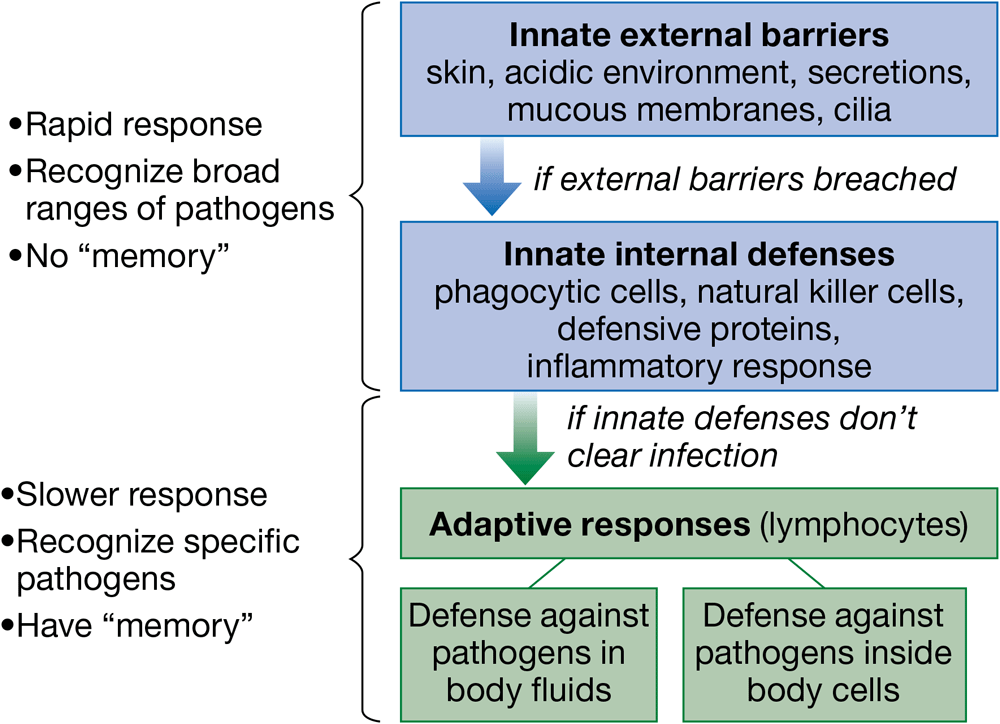
\includegraphics[width=0.4\textwidth]{response_table.png}
	\end{center}
	\caption{Various types of immune responses}
\end{wrapfigure}

In contrast to the more general innate immune mechanisms that have been defined
thus far, \textbf{adaptive immunity} or \emph{acquired immunity} describes an
immune response that is highly specialized in its target pathogen, and is
activated only \emph{after} exposure to a pathogen. Generally, an adaptive
immune response is triggered by a pathogen, but adaptive responses are not
limited \textbf{only} pathogens. As such, when a molecule triggers an adaptive
immune response, it is referred to as an \textbf{antigen}. Keeping in mind this
naming scheme, we can refer to a countering protein originating from blood plasma
as an ``\textbf{antibody}'' (antigen = antibody-generating). Due to the
specialized nature of adaptive immune responses, antibodies are only effective
with consideration to the antigen for which they were produced.

Though exposure to antigens is generally the principal mechanism by which
antibodies are produced, antibodies can be obtained for a specific pathogen by
inducing an adaptive immune response through, for example, vaccination. Both
natural and artificial adaptive immune responses, resulting in the production
of antibodies for a desired antigen are considered forms of \textbf{active
immmunity}, as they require an individual's immune system to produce antibodies
on its own behalf. \textbf{Passive immunity}, on the other hand, is obtained
when premade antibodies are given to an organism (e.g., through the placenta or
breast milk).

The name \textbf{lymphocyte} is given to a white blood cell responsible for
this type of immunity, adaptive immunity---be it artificially or naturally
induced adaptive immunity.

\section{The lymphatic system}

In both the case of innate and adaptive immunity, the \textbf{lymphatic system}
serves as an instrumental component to the survival of the organism in
question. More specifically, the lymphatic system serves as a ``filter'' for
infectious material, and, as such, has two main functions:

\begin{enumerate}
	\item fighting infection
	\item returning tissue fluid to the circulatory system
\end{enumerate}

The lymphatic system is composed of various \textbf{lymph nodes}---masses of
lymphocytes and macrophages---and \textbf{lymphatic vessels} which contain
\textbf{lymph}. The latter of these structures, the lympatic vessel, serves
to return fluid to the blood after filtration---specifically, to the
circulatory system through vessels that fuse with veins in the chest.
The former, on the other hand---the lymph node---aids in the circulation of
lymph, which carries various toxins picked up from infection sites in the body.
Once lymph has circulated to each of the lymph organs, macrophages are able to
ingest the unwanted material as part of the body's immune response.

\subsection{Types of lymphocytes}

As was previously mentioned, \textbf{lymphocyte} are responsible for adaptive
immunity. However, even within the disambiguation, ``lymphocyte'', there
exists two specialized kinds of defensive cells: B cells and T cells.
However, each of these kinds of cells are derived from the general
classification, ``lymphocyte'', and are differentiated from immature stem cells
inside their respective housings---the bone marrow for B cells, and the thymus
for the T cell.

Each of these cells serve different purposes, and are specialized for specific
kinds of infections. More specifically, the T cell is responsible for what is
termed the ``cell-mediated immune response''---action against infected cells.
B cells, on the other hand, are responsible for the ``humoral immune response''
---action against free-floating antigens.

Generally, the humoral and cell-mediated immune responses can be described in
terms of the pathogen or antigen that they target. In other words, we can
define the humoral and cell-mediated responses as such:

\begin{itemize}
	\item \textbf{Humoral immune response}: targets bacteria and viruses in the
		body fluids. Results in the secretion of free-floating antibodies into
		the lymph and blood
	\item \textbf{Cell-Mediated immune response}: defends against infections
		inside body cells. Results in the destruction of body cells infected
		with bacteria or viruses.
\end{itemize}

As has been recognized thus far, the general term ``lymphocyte'' can be used to
refer to a T cell or a B cell. However, the disambiguation ``T cell'' in and
of itself can be further divided into more specific categories. For example,
the defensive T cell functions directly in the humoral immune response by
ingesting infected body cells. Other T cells might simply promote phagocytosis,
rather than defensive T processes.

\subsection{Structure of a lymphocyte}

In the process of differentiation, protein molecules are attached to the
surface of a lymphocyte. These proteins are \textbf{antigen receptors}, which
allow a lymphocyte to bind to a specific type of antigen. Usually, antibodies
released as a result of a lymphocyte's actions will bind on to the
\textbf{epitope} of the antigen at the lymphocyte's
\textbf{antigen-binding site}, which has a shape complementary to that of the
epitope.

Keeping in mind that antigen receptors are attached to B and T cells before
contact is ever made with the target antigen, a large variety of lymphocytes
exist in most humans.

Once the structure of a lymphocyte has developed, resulting in differentiation,
a lymphocyte must be expelled to the bloodstream and to the spleen, lymph
nodes, and the lymphatic system.

\begin{figure}[h]
	\centering
	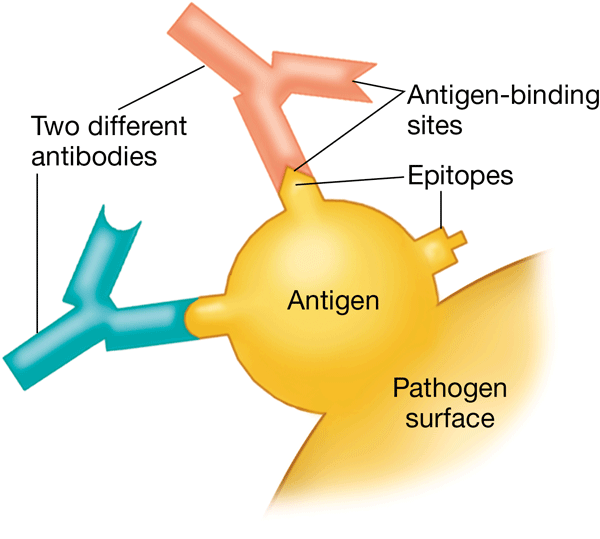
\includegraphics[width=6cm]{antigen_lymphocyte_binding.png}
	\caption{Antibodies binding on to an epitope.}
\end{figure}

\subsection{Clonal selection as a result of lymphocyte binding}

\subsubsection{Types of clonal lymphocyte binding cells}

Once a lymphocyte cell binds to an antigen, the cell proliferates, forming
various clones of cells capable of responding to the aforementioned antigen.

Of these ``clone'' cells, two categories exist: \textbf{effector cells} that
take effect immediately, neutralizing an infectious agent, and \textbf{memory}
cells that wait for the next encounter with such an agent.

\begin{figure}[h]
	\centering
	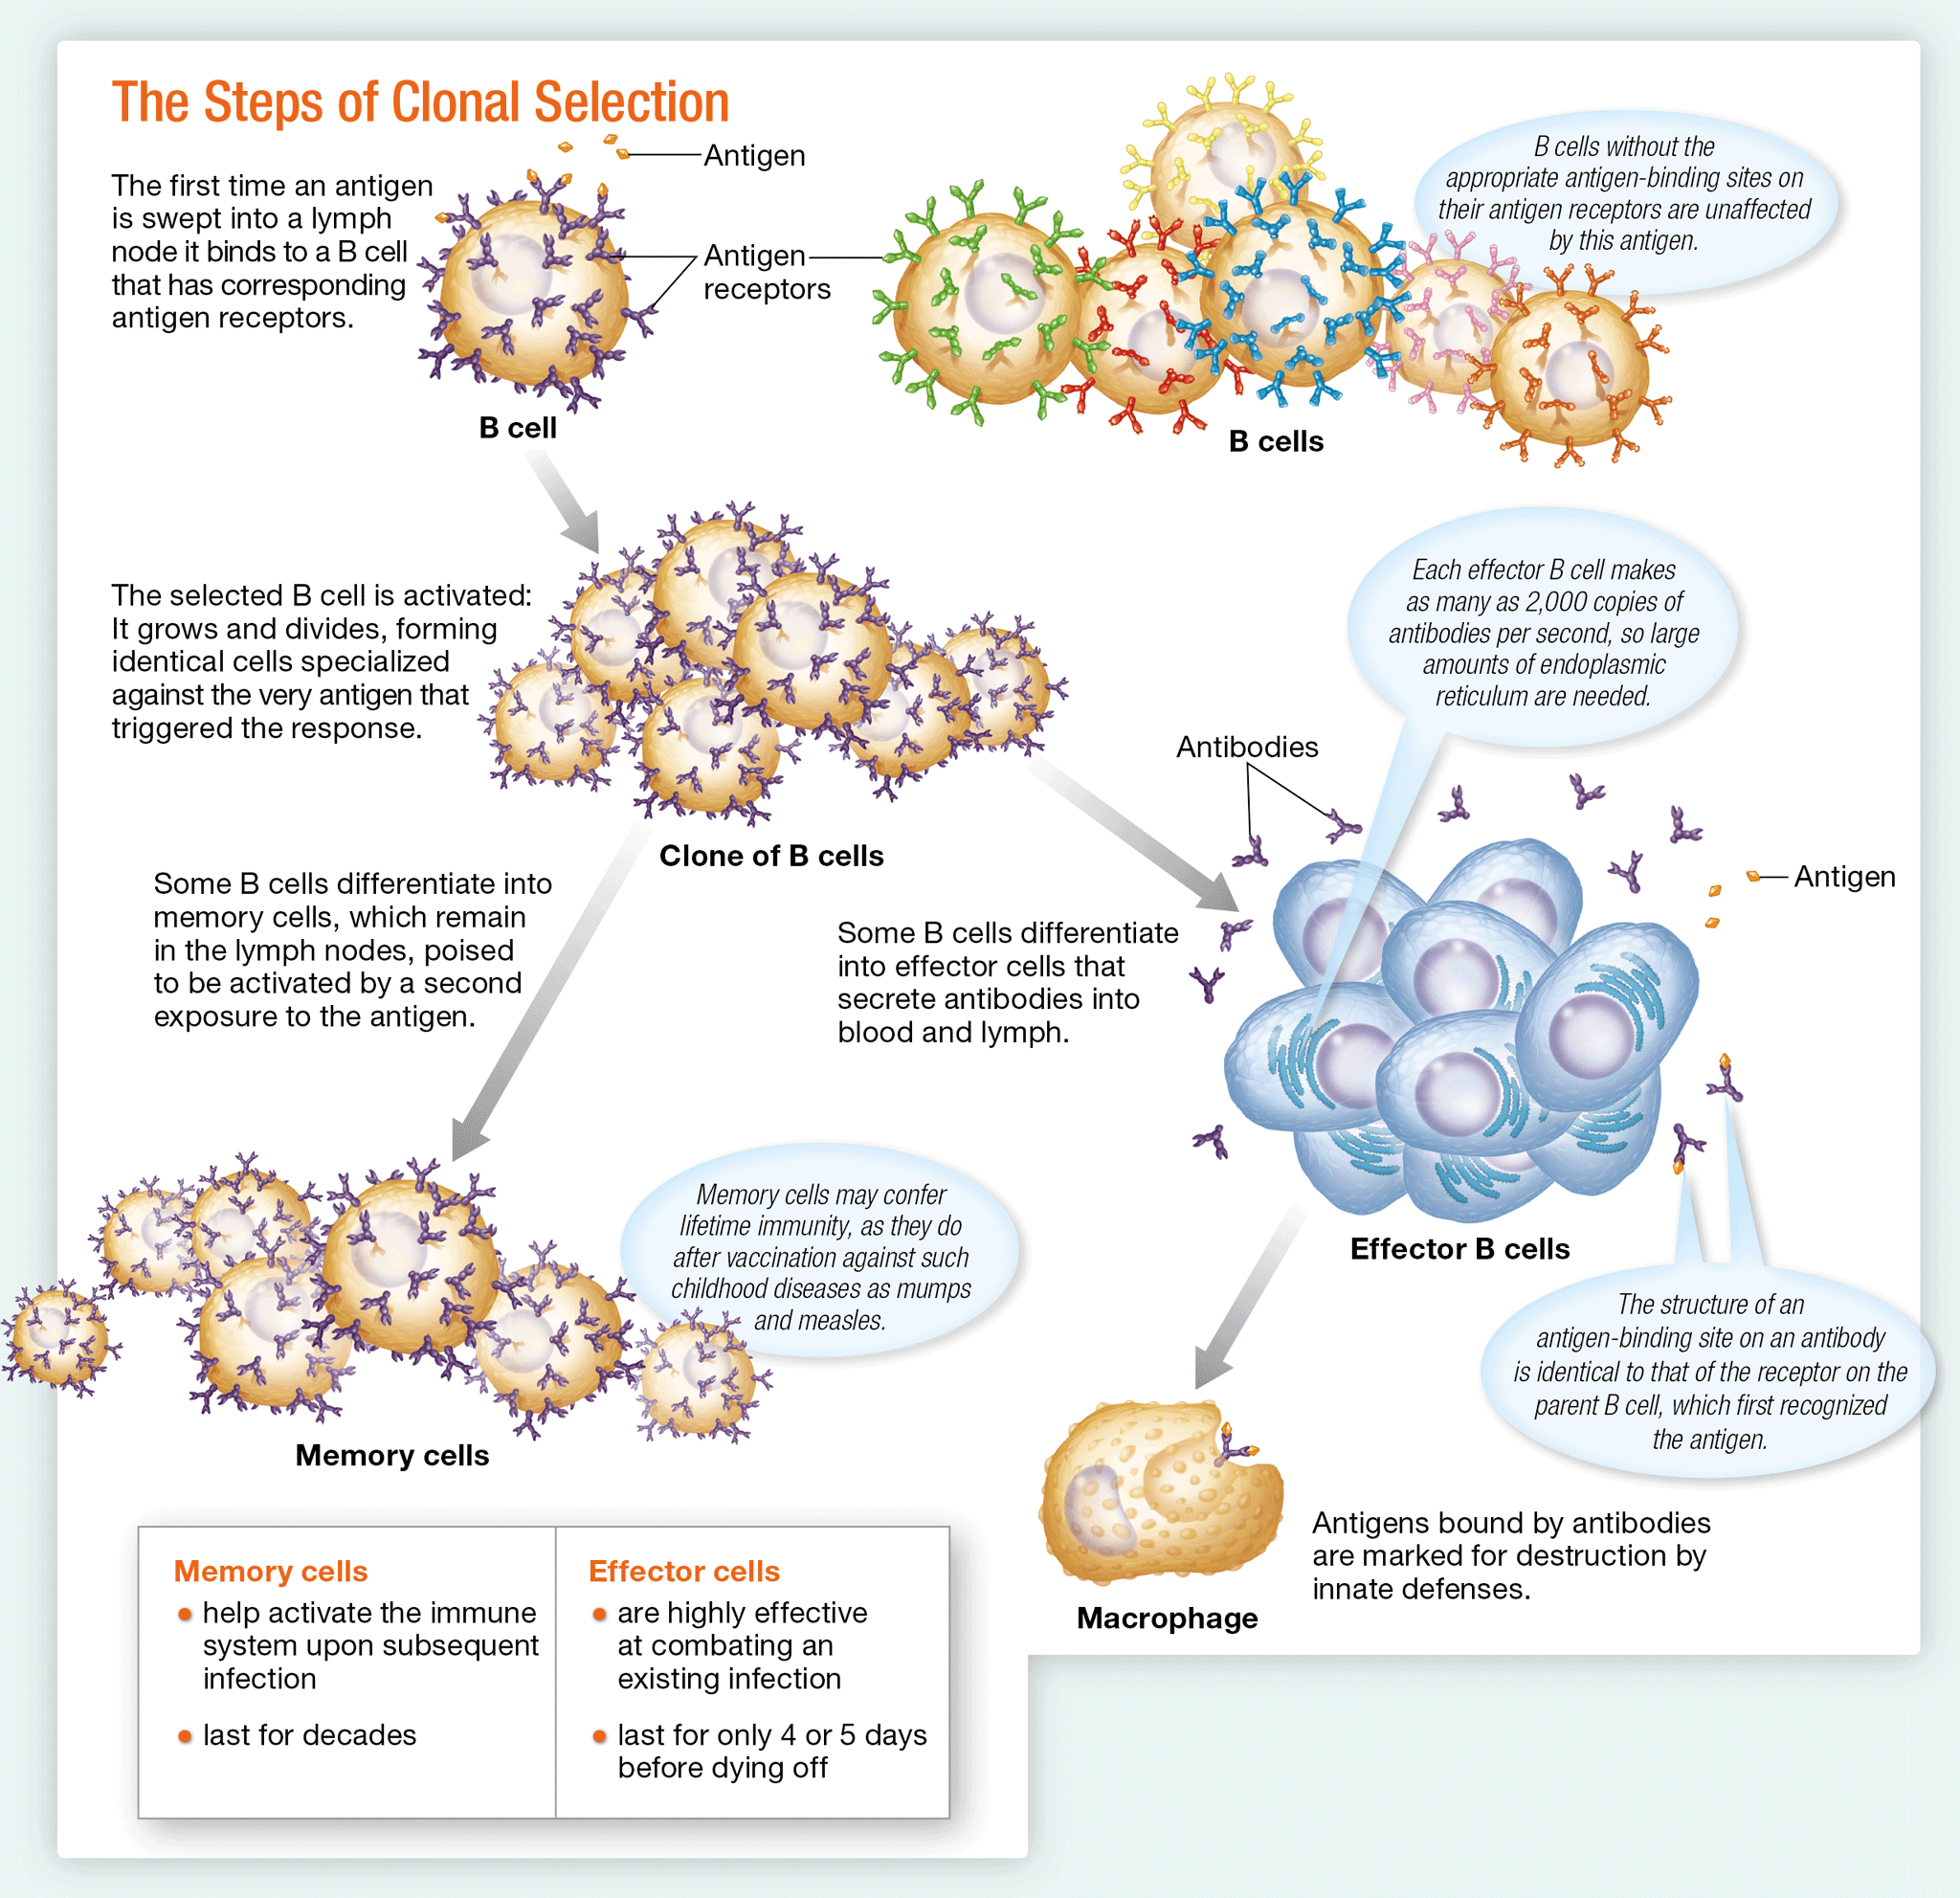
\includegraphics[width=12cm]{lymphocyte_clone_cells.png}
	\caption{The process by which ``selected'' cells are cloned}
\end{figure}

\subsubsection{Differences between the primary and secondary responses}

\begin{wrapfigure}{r}{0.4\textwidth}
	\centering
	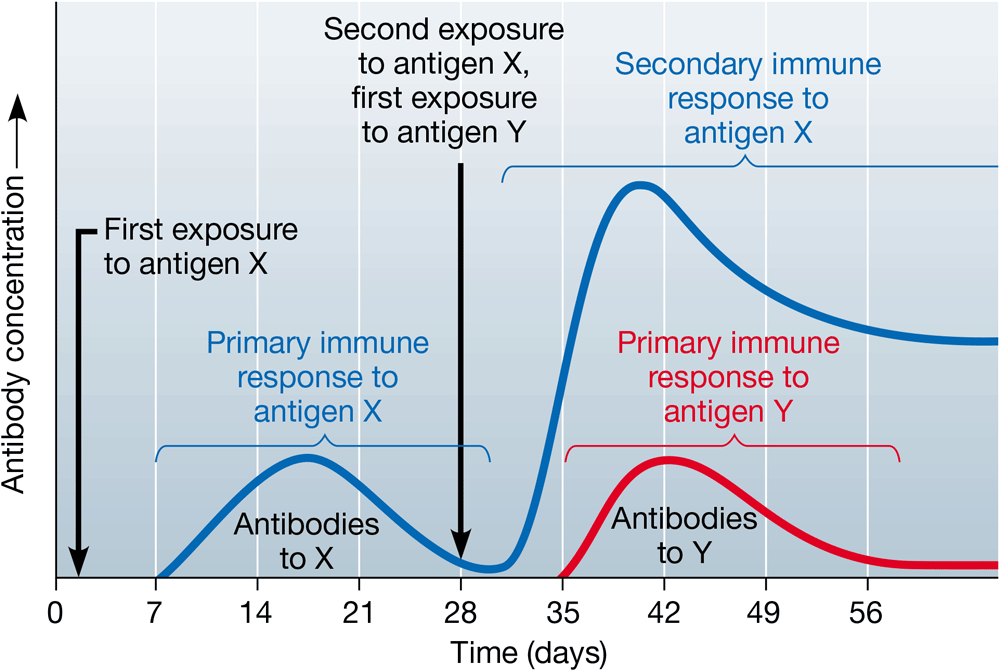
\includegraphics[width=0.4\textwidth]{primary_vs_secondary_response_graph.png}
\end{wrapfigure}

As is suggested by the nature of the aforementioned ``cloning'' process,
generating a sufficient number of ``selecting'' cloned cells at the primary
immune response takes a significantly longer amount of time than in the case
of a sequential response---the secondary immune response. This is caused by
the fact that, once an infectious agent has arrived within an organism, enoguh
``cloned'' cells have been produced for the same response to be evoked without
waiting for the production of such ``cloned'' selecting cells on the next
encounter with an effective agent. In other words, these ``selecting'' cells
are stockpiled, in hopes that, when an agent is next encountered, there will be
a sufficient quantity to neutralize the threat.

\section{The role of antibodies in immunity}

\subsection{The structure of an antibody}

An important distinction must be made between the role of an antibody and, for
example, a B or T cell. Or, that is to say that a common misconception lies in
the function of the antibody. An antibody does not serve to harm an infectious
agent. But, rather, an antibody simply ``marks'' an agent for destruction. The
action of agent destruction is carried out by various other components of the
immune system, but not by the antibody. Again, by forming a chemical bond
between the \emph{antigen-binding site}, antibodies simply form a complex that
can be easily recognized by other components in the immune system.

More specifically, the role of the antibody in the humoral immune response is
twofold:

\begin{enumerate}
	\item Recognizing and binding to an antigen
	\item Assisting in---but not necessarily carrying out---the elimination of
		such an antigen
\end{enumerate}

The antibody satisfies these stipulations not by function, but as a side-effect
of its structure: each antibody consiss of four Y-shaped polypeptide complexes.

\begin{figure}[h]
	\centering
	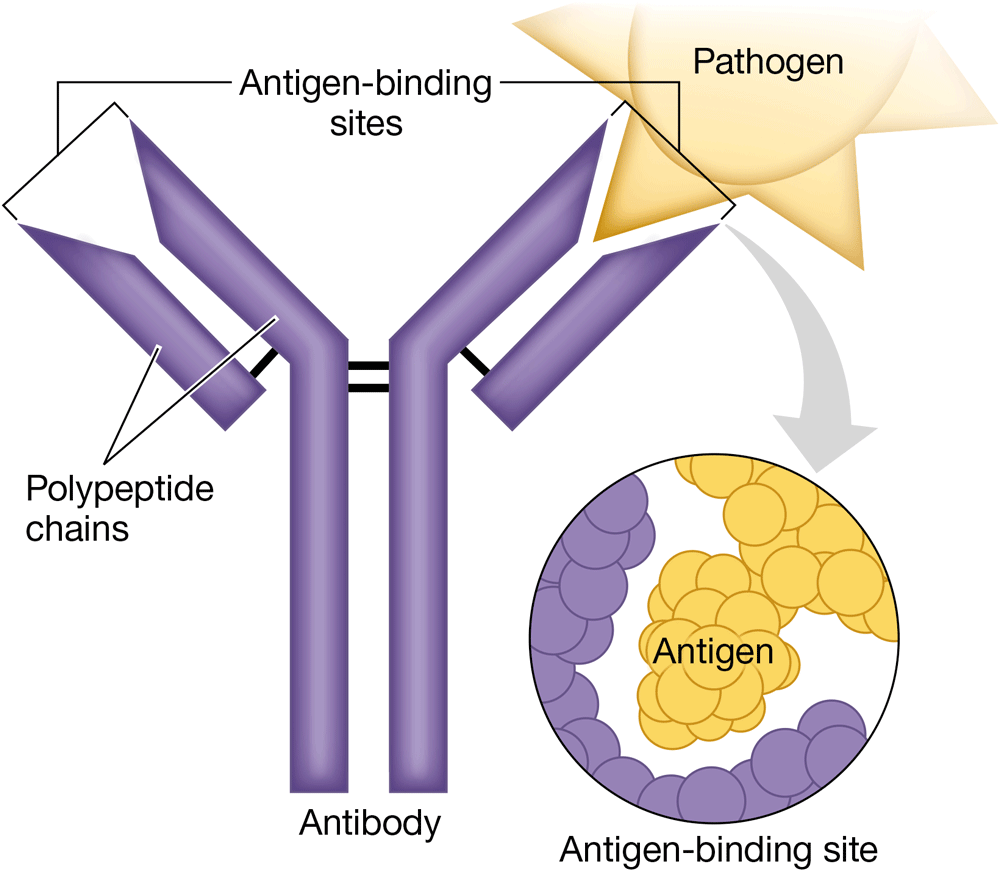
\includegraphics[width=8cm]{antibody_structure.png}
	\caption{The structure of a typical antibody.}
\end{figure}

\subsection{Components of the innate immune system can work in conjunction with specific recognition}

\begin{wrapfigure}{r}{0.5\textwidth}
	\centering
	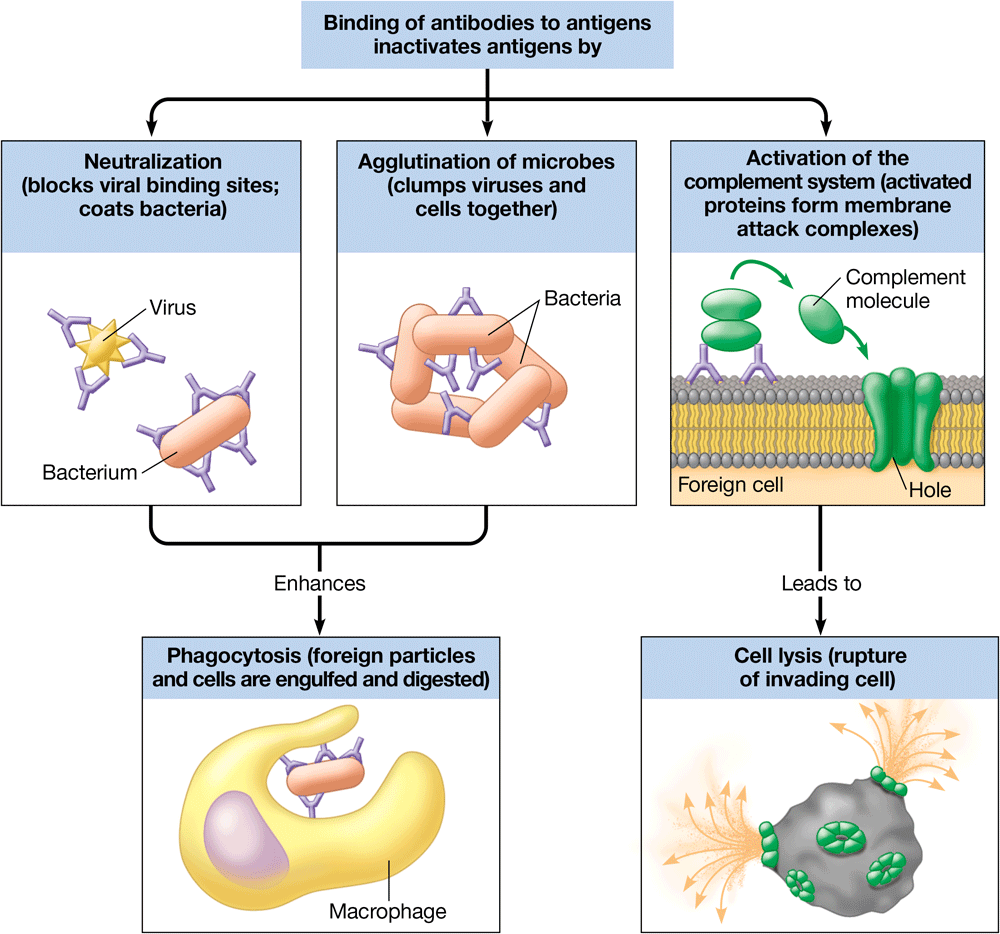
\includegraphics[width=0.7\linewidth]{innate_destruction.png}
\end{wrapfigure}

In order to dispose of an infectious agent, the humoral immune response must
look to the innate immune system: the complement system and macrophages are
responsible for attacking invading agents. More specifically, during the
neutralization phase, antibodies bind to the agent, letting macrophage cells
easily recognize the intruding entity. Of course, this results in the ingestion
of the agent by a macrophage. However, the macrophage is not the sole path to
the destruction of a harmful agent: once activated as a result of antibody
bindings, members of the complement system can act to ``poke holes'' in the
membrane of the invading cell or agent, causing it to swell and lyse.

\section{Helper and cytotoxic T cells}

\begin{wrapfigure}{r}{0.4\linewidth}
	\centering
	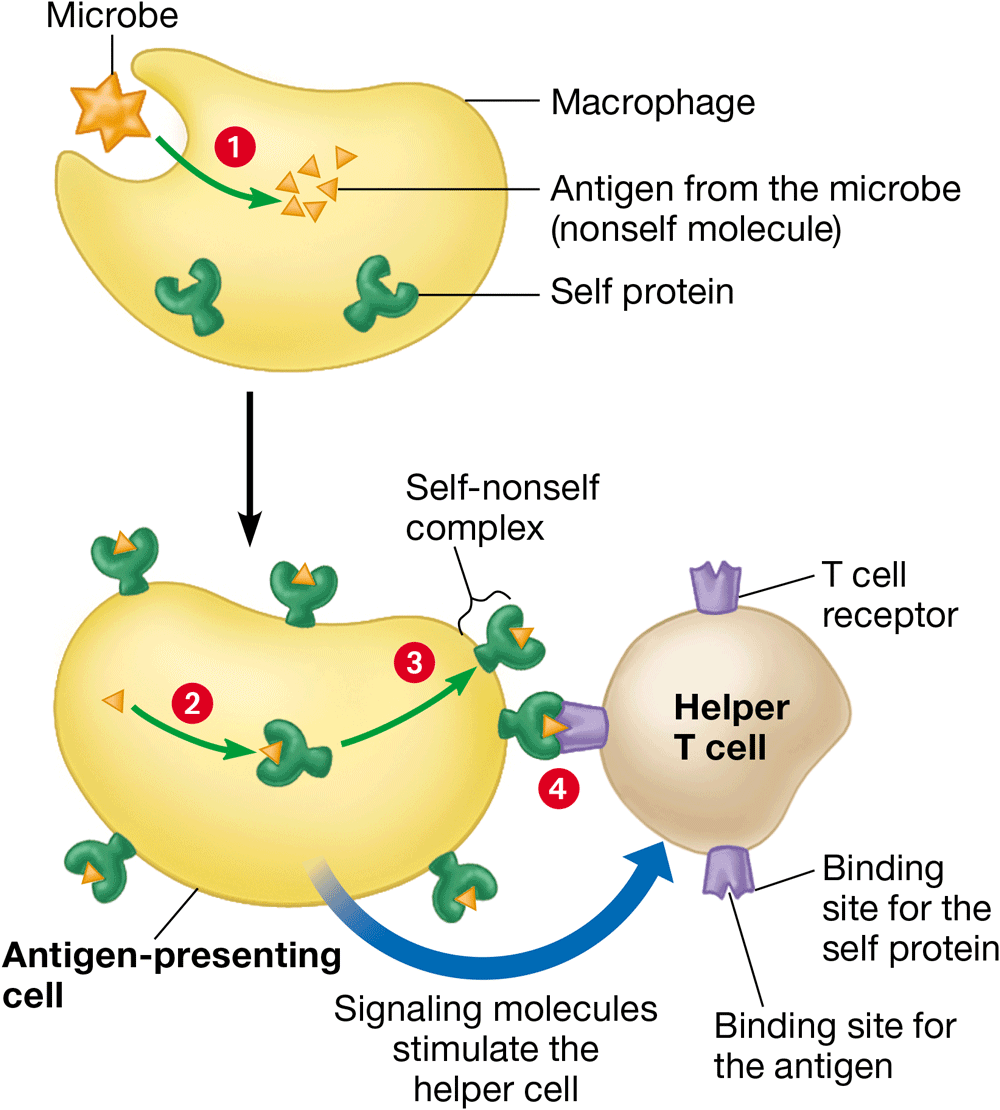
\includegraphics[width=1\linewidth]{self_nonself_complex.png}
	\bigbreak{}
	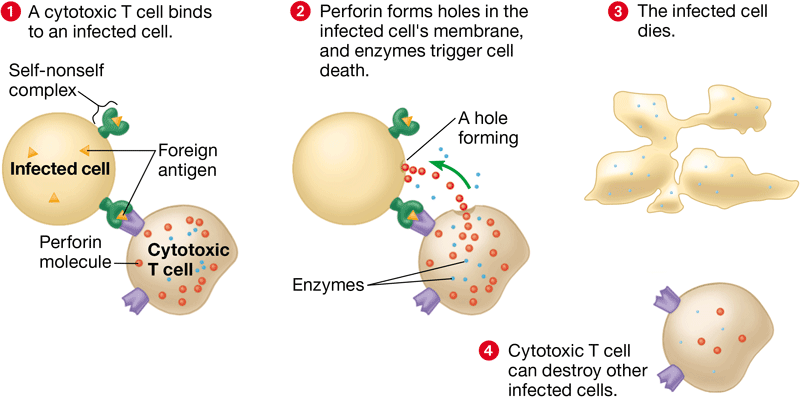
\includegraphics[width=8cm]{cytotoxic_t_cell.png}
	\caption{Self-nonself recognition (top), Agent breakdown (bottom)}
\end{wrapfigure}

Once a pathogen has entered a body cell, the cell-mediated immune response
produced by the ``cytotoxic T cell'' must battle the pathogen. However,
cytotoxic T cells don't act of their own volition. But, rather, a
\textbf{helper T cell} triggers the humoral and cell-mediated immune responses
by signaling to initiate the production of antibodies that neutralize pathogens
or activate cytotoxic T cells. In other words, the helper T cell is essentially
a central coordinator for the entire immune system---that is, excluding
external innate barriers. Without helper T cells, no immune response is evoked
from the body outside its autonomous, innate, external barrier functions---
which are, of course, not functional, but structural in their utility.

In order for a helper T cell to activate, several requirements must be met:

\begin{itemize}
	\item The antigen receptor of the T cell must be active---that is, it must
		be able to bind to the agent or molecule in question
	\item The antigen must be displayed on the surface of an antigen-presenting
		cell (e.g., marcophages, B cells)
\end{itemize}

In practice, these requirements could be met in the following sequecne of
events:

\begin{enumerate}
	\item A macrophage ingests a foreign particle and breaks the particle into
		its foreign antigens
	\item \textbf{Self proteins}, or proteins belonging to the macrophage bind
		to the foreign antigens
	\item The macrophage display a \textbf{self-nonself complex}---a
		combination of the self protein and the foreign antigen---on its
		surface
	\item A helper T cell recognizes the self-nonself complex
\end{enumerate}

\end{document}
